\documentclass{listhesis}
% --- Listhesis builds on KOMA script report (scrreprt).
%     Class arguments are passed to that class.

% --- Add additional packages here using \usepackage{package-name}.

% --- Provide your thesis details here.
\setup{%
  % de,                   % uncomment if your thesis is in German
  author=Iffat Brekhna, % your name
  title={Simulator Support for Dynamic Data Migration on a Distributed Shared Memory Architecture},
  date={June 21, 2018}, % submission date (today is used if unset)
  type=master,        % thesis type [master, bachelor, research, internship, diplom]
  advisor=Sven Rheindt M.Sc, % your advisor (typically some PhD. student)
  supervisor=Prof. Dr. sc. techn. Andreas Herkersdorf, % your supervisor
  % % uncomment the next lines if your thesis was carried out in industry
  % company=External Company,
  % externalAdvisor=Your Companyadvisor
}

\begin{document}
\maketitle
\cleardoublepage

% --- Thesis abstract.
%     For German thesis also provide an English version via the optional
%     argument: \anstract[English]{German}
\abstract{


Current processor architectures have shifted from microarchitecture to macroarchitecture which implies that processors with multiple tiles and cores are introduced. These processors have non-uniform memory access (NUMA) properties where the memory access time depends on how close the memory (data) and tasks (cores) are located. In order to reduce the distance between the tasks and data, processors which have a distributed-shared memory architecture are introduced where the memory is distributed and shared among all the tiles. To study the effects on performance of a data and/or task management techniques we need to have simulator support for such schemes in the existing simulator. In this thesis the simulator support for a dynamic data migration (DDM) scheme is build into the current simulator and it's performance is evaluated. DDM migrates data at run time from one location to another so that the distance between the tasks and data is reduced. With a block size of four cache lines, a time interval of 500 nsec and no data placement we gained a speed up of 46\% and 48\% with DDM on compared to no dynamic data migration for blackscholes and canneal respectively.
}
\makeabstract
\clearpage

% --- Content tables.
\tableofcontents
\clearpage
\listoffigures
\clearpage
\listoftables
\clearpage

% --- Your thesis starts here.
%     Use \chapter{}, \section{}, \subsection{}, \subsubsection{},
%     and \paragraph{} to structure your thesis.

\chapter{Introduction}
\section{Motivation}
\subsection{Power Wall}
In a single core system, the speed of the processor is determined by its frequency. Hence, increasing the processor's speed means to increase its operating frequency which in terms increases the power dissipation. The bottleneck here is the \textit{power density} which is the power per die area. With increasing frequency a point is reached when the power density is similar to that of a core of a nuclear reactor and if we extrapolate the graph we reach to the power density of that inside a rocket nozzle. This makes it quite challenging to dissipate the heat and run the system efficiently. Hence, a maximum frequency is reached due to the limitations on power dissipations. This scenario is called the \textit{power wall} as shown in figure~\ref{fig:powerwall}. The solution to this is to use multiple cores at a frequency which gives feasible power dissipations in-order to achieve high computing speeds which gave rise to multi-core computing.\\
\begin{figure}[h!]
  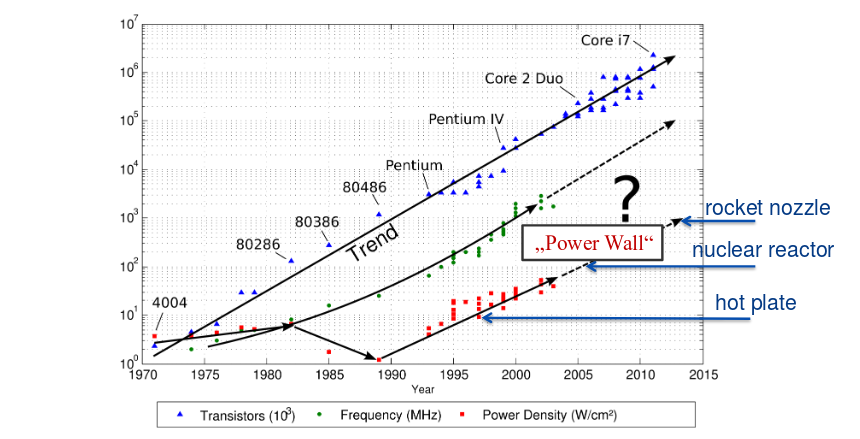
\includegraphics[width=\linewidth]{powerwall.png}
  \centering
  \caption{Power Wall~\cite{chipmulticore}}
  \label{fig:powerwall}
\end{figure}
\subsection{Memory Wall}
The \textit{memory wall} is a situation where the improvement of the speed of dynamic random access memory (DRAM) does not scale with the fast improvement of the processor speed hence resulting in a gap between the two technologies which lowers the speeds of the overall system~\cite{memorywall}. It is illustrated in figure~\ref{fig:memorywall}. You can see in the figure that there is a gap between the improvements in processor performance and memory performance which is increasing with time. We need to bridge this gap in order to speed up processors and hence the concept of caches and memory management techniques are introduced.\\
\begin{figure}[h!]
  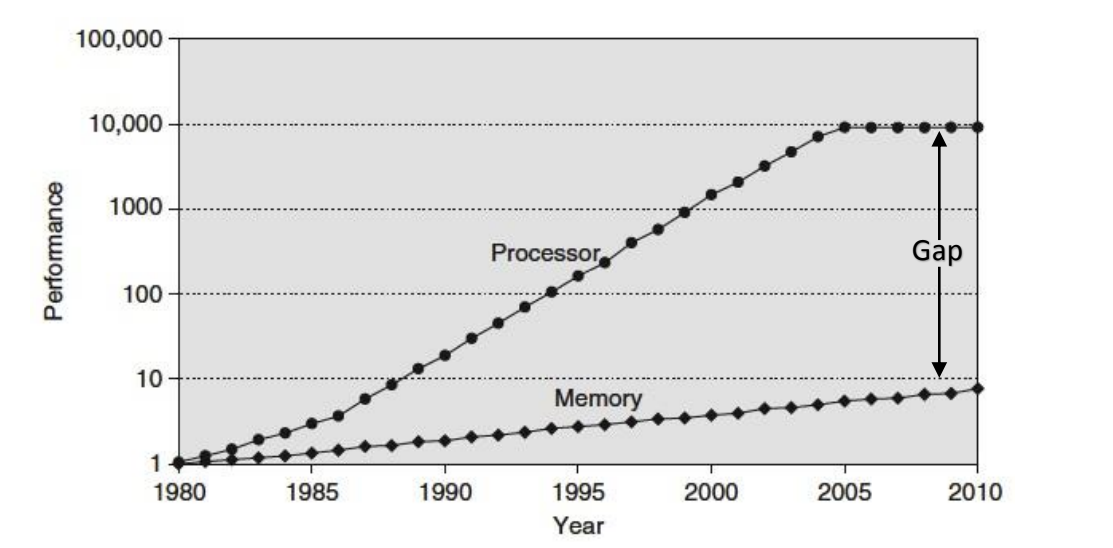
\includegraphics[width=\linewidth]{memorywall.png}
  \centering
  \caption{Memory Wall~\cite{hennessy}}
  \label{fig:memorywall}
\end{figure}
\\
Due to the memory wall and power wall described above current research in semi-conductor industry is towards developing a single chip multi-tile multi-core processor. Hence, parallel programming is experiencing a rapid growth with the advent of system on chip (SoC) architectures. One example of such a system is the Invasic architecture~\cite{invasive} as shown in Figure \ref{fig:multi-core,tile}. The main idea of Invasic architecture is to introduce ``resource aware programming" support so that a program has the ability to explore its surroundings and dynamically spread its computations to neighboring processors~\cite{invasive}. Because of multiple tiles and cores on one chip these processors deal with data processing at a high scale and complexity. Therefore, the bottleneck has shifted from computational complexities to data management techniques.\\
\\
Modern, scalable multiprocessor system-on-chip (MPSoC) platform's memory access time depends on where the memory is located relative to the core which accesses the memory. In other words (MPSoC) platform's have Non-Uniform Memory Access (NUMA) properties because it has a distributed shared memory (DSM) architecture, hence application performance is highly influenced by data-to-task locality~\cite{sven, lispaper}. The goal is to bring tasks and data closer together to increase overall performance. This is a twofold and complementary problem consisting of data and or task migration. In this thesis, we will look into data migration and see how it improves the performance of the MPSoC.\\
\\
We propose a dynamic data migration (DDM) scheme in which the data is migrated dynamically at run time from one Tile Local Memory (TLM) or DDR to another TLM or DDR if the need arises. This is the major differentiating factor of our approach from the current research in the group; managing data placement at run time rather than at compile time.
\section{Problem}
In~\cite{lispaper} the research in the group has been described. The authors explain how data is placed on the TLM. They divide the data used by an application at the granularity of memory pages and place them on the local memory according to the ideal location that is derived based on the task-to-data mapping techniques. They propose two techniques on how to do this task-to-data mapping:\\
\par
\textit{First Touch Policy}: As the names suggest, in first touch the memory blocks are migrated to the TLM of the tile that accesses the data first~\cite{lispaper}. The drawback of first touch policy is that data can be placed at a local memory far away from the core that accesses it frequently hence increasing the memory access time. You cannot change the location of data at run time even if it is giving performance disadvantages.\\ 
\par
\textit{Most Accesses Policy}: In most accessed the memory blocks are migrated to the TLM of the tile that accesses it the most over the complete application~\cite{lispaper}. The drawback of the most access policy is that the evaluation is performed for a complete application's runtime so data cannot be migrated dynamically at run time but instead it is only placed statically at compile time. Also, it is a unrealistic scenario since the whole trace-file is needed at compile time. 
\begin{figure}[h!]
  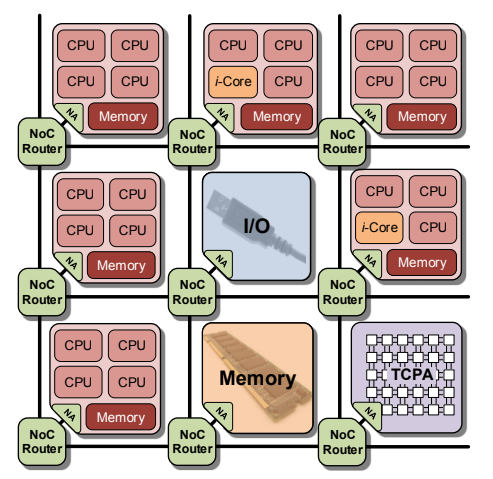
\includegraphics[width=0.7\linewidth]{multi-core,tile.png}
  \centering
  \caption{Invasic Architecture~\cite{iNetworkAdapter}}
  \label{fig:multi-core,tile}
\end{figure}
\section{Goals of Thesis}
The goal of this thesis is to design, implement and evaluate a dynamic data migration technique for memory management at run time for a trace-based simulator. The system will evaluate itself repetitively and find the best data placement to improve it's performance. \\
\\
The outcome will be a system which does not need external support to find the best placement for its memory but rather it will adapt itself to migrate the data at the best location which will hopefully improve the performance. 
\section{Approach}
The steps followed to develop the Simulator Support for Dynamic Data Migration are as follows:
\begin{itemize}
  \item Understanding the Idea: In this step, the purpose is to understand why we need data migration in the first place and how data placement is done statically on a distributed shared memory system. We look into other means of bringing the data close to the processor as well. 
  \item Literature Review: Find and read relevant work that has already been done for bringing the data and process/task together. Choose one approach on how to bring data and task together and find relevant ideas to understanding the concept better. 
  \item Design: Here we decide which technologies to use and how to design our system for optimal results. We want a design that is easy to change, extend, optimize and is scalable. Also, we decide how we will evaluate our system eventually and what metrics we will use in result gathering. 
  \item Implementation: Implement the design of the solution. 
  \item Evaluation and Testing: Compare the performance of dynamic data migration with static data placement techniques.
\end{itemize}
\section{Outline}
The work is structured as follows. In Chapter 1 a brief introduction of the problem is given along with the motivation to solve it and then a brief overview of the solution is given.
In Chapter 2 the basic concepts needed to understand how dynamic data migration is implemented are explained along with the work already done related to this thesis is given. In Chapter 3 the system architecture is introduced i.e the modules added for implementing dynamic data migration are introduced and explained. In Chapter 4 the implementation is explained in detail. In Chapter 5 the the programs that assisted or were used for running the simulations before gathering results are given. In Chapter 6 the results are presented. It shows how the performance has changed with the proposed solution implementation. In Chapter 7 a summary is given along with some suggestions for future works in this domain. 
\chapter{Background and Related Work}
In this chapter the necessary background information is introduced in order to understand the thesis. Moreover, we will discuss the related work in this domain of research.\\
\\
\section{Basic Concepts}
\subsection{Tile}
Figure \ref{fig:tile} shows a single tile. You can see in the figure that it composes of four cores, L1 caches for every core, L2 cache which is shared between all the cores and a Tile Local Memory (TLM) which is also shared by all the cores. It also has a Bus which connects the cores to the L2 Cache and the TLM. Each component of the tile is explained below.
\par
\textbf{Core}: A Core is the basic processing unit that receives instructions (from the user or application) and performs calculations based on those instructions. A processor can have a single core or multiple cores.  
\par
\textbf{TLM}: TLM stands for Tile Local Memory. Each tile has its own TLM which is shared among all the Cores of the tile~\cite{ankitThesis, iNetworkAdapter}. This memory is cachable by the L1 caches of all the Cores within the tile that it sits on and by the L2 cache of any other tile. The TLM from one tile can be accessed by the core of another tile.
\par
\textbf{Bus}: The bus connects the Core to the L2 Cache and the TLM. Also, when another tile has to be accessed the request goes through the bus to the network adapter.
\par
\textbf{Network Adapter (NA)}: The network adapter provides the interface between a tile and the network connection which is providing a connection to other tiles and the DDR.
\par
\textbf{Load Store Unit (LSU)}: The Load-Store Unit (LSU) is a communication path between different modules. It's main function is to receive, process and retransmit different requests from the modules that are connected to it.
\par
\textbf{Cache}: Cache is a temporary storage space which is made up of high-speed static RAM (sRAM). It stores information which has been recently accessed so that it can be quickly accessed at a later time. It operates on the principle that most programs access information or data over and over again so by having data in the SRAM the CPU does not access the slow DDR/DRAM again and again. A cache hit occurs when the processor core accesses data that is already present in the cache whereas a cache miss occurs when the data is not present in the cache and has to be fetched from the TLM or the main memory to the cache. In our architecture we have two levels of caches:
\begin{itemize}
  \item L1 Cache: Level 1 cache (L1 Cache) is the cache right next to the core and is the smallest in size. It is not shared with any other core i.e it is a private cache.
  \item L2 Cache: Level 2 cache (L2 Cache) is away from the processor and is larger in size than the L1 cache. It is shared between all the cores in a tile. In our scenario, L2 cache is the Last Level Cache (LLC) in the system.
\end{itemize}
\begin{figure}
  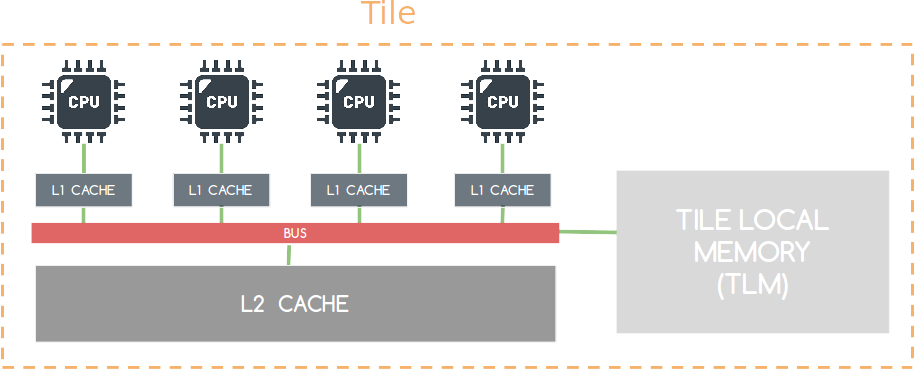
\includegraphics[width=\linewidth]{tile.png}
  \centering
  \caption{A Tile}
  \label{fig:tile}
\end{figure}
\section{Related Work}
The main idea is to bring data and tasks close together in order to save execution time used in transferring data back and forth. This can be achieved in several ways. The data can be brought closer to the tasks by caching it in the cache of the core accessing it or by migrating tasks to data instead. Also, we can migrate data to the local memory near the core accessing the data. These different ideas on how it has been done are discussed in the subsections below. 
\subsection{Data Placement/Migration on Caches}
This section explicitly talks about how data placement and migration has been implemented in caches for a Non-Uniform Cache Access (NUCA) architecture. A great amount of work has been done on data-placement in the shared last level cache (LLC) in order to reduce the distance of data from the core requesting the data and to take care of load balancing across the chip.\\
\\
In static data placement~\cite{cacheDataPlacement1, cacheDataPlacement2} the whole address space is divided into subsets and every subset is mapped to a LLC slice regardless of the location of the requesting core which leads to unnecessary on-chip traffic. Its advantage is that it evenly distributes the data among the available LLC slices and reduces off-chip accesses. In dynamic data placement~\cite{cacheDataPlacement1, cacheDataPlacement3, cacheDataPlacement4} the data blocks are placed such as to reduce the distance between the data block's home node and the core requesting it. This eliminates the unnecessary on-chip traffic. It requires a lookup mechanism to locate the dynamically selected home node for each data block. In reactive data placement data is classified as private or shared using the operating systems page tables at page granularity~\cite{cacheDataPlacement4},~\cite{cacheDataPlacement6}. Because all placement is performed at page granularity level there is load imbalance as some LLC slices might have higher accesses compared to others. This load imbalance leads to hot-spots~\cite{cacheDataPlacement6}.\\
\\
There is a hybrid data placement~\cite{cacheDataPlacement6} which combines the best features of static and dynamic data placement techniques. It optimizes data locality and also takes care of load balancing of the shared data. Hybrid data placement differs from Reactive data placement in regard to allocation of shared data among the cores i.e in Hybrid data placement, data is also classified as private or shared using the operating systems page tables but when a page is classified as shared (in hybrid data placement) it is allocated to a cluster of LLC slices and within this cluster the page is statically interleaved at the granularity of cache lines~\cite{cacheDataPlacement6}. This balances the load among the LLC slices.\\
\subsection{Task/Thread Placement}
Placing threads that share data on the same core improves performance~\cite{threadPlacement1}. However, finding the optimal mapping between threads and cores is a NP-hard problem~\cite{threadPlacement2} and cannot be scaled. One way to solve this problem is by monitoring the data accesses to determine the interaction between threads and the demands on cache memory~\cite{threadPlacement3}. In~\cite{threadPlacement3} a mechanism is there to transform the number of memory accesses from different threads to communication patterns and use these patterns to place the threads that share data on cores that share levels of cache.  They generate a communication matrix using the number of accesses to the same memory location by two threads and then maps the threads with highest communication to the same core. The disadvantage of this method is that generating the communication matrix through simulation is slow and they propose the application vendor provides this matrix with the application.\\
\\
In~\cite{threadPlacement4} a thread scheduling mechanism is proposed which uses the performance monitoring unit (PMU) with integrated hardware performance counters (HPCs) available in today's processors to automatically re-cluster threads online. Using HPSs they monitor the stall breakdowns to check if cross chip communication is the reason for the stalls. If that is so, they detect the sharing pattern between the threads using the data sampling feature of the PMU.  For every thread they maintain a summary vector called the shMap  which holds the signature of data regions accessed by the thread which resulted in cross-chip communication. These shMaps are analyzed i.e threads with high degree of sharing will have similar shMaps and will be placed to the same cluster. The OS then migrates the threads with higher sharing to the same cluster and place them as close as possible~\cite{threadPlacement4}.\\
\subsection{Data and Thread Migration}
In~\cite{datathreadPlacement} a mechanism called CDCS is presented which using a combination of hardware and software techniques jointly places threads and data in multi-cores with distributed shared caches. CDCS takes a multi-step approach to solve the various interdependencies. It places data first and then places threads such that the threads are close to the center of mass of their data. Then using the thread placement it again re-place the data and once again for this data it re-places the threads to get a optimum placement. This technique improves performance and energy efficiency for both thread clustering and NUCA techniques~\cite{datathreadPlacement}.\\
\subsection{Data Placement on TLM}
This section talks about the data placement mechanisms for the NUMA architecture.
\subsubsection{Static Data Placement on TLM}
In~\cite{lispaper} the authors have implemented static data placement for the distributed-shared memory in a NUMA architecture system. They divide the data used by an application at the granularity of memory pages and migrate it from the global memory to the local memory according to a ideal location that is derived based on the task-to-data mapping techniques. They propose two schemes on how to do this task-to-data mapping:\\
\par
\textbf{First Touch Policy}: As the names suggest in First Touch Policy the memory blocks are migrated to the TLM of the tile that accesses the data first. The drawback of first touch policy is that data can be placed at a local memory far away from the core that accesses it frequently hence increasing the memory access time. You cannot change the location of data at run time even if it is giving performance disadvantages.\\  
\par
\textbf{Most Accesses Policy}: In Most Accessed Policy the memory blocks are migrated to the TLM of the tile that accesses it the most over the complete application runtime. The drawback of this policy is that the evaluation is performed for a complete application's runtime so data cannot be migrated dynamically at run time but instead it is only migrated statically at compile time.
\subsubsection{Dynamic Data Placement and Migration on TLM}
In~\cite{dynamicPageMigration},~\cite{dynamicpMigration} the authors have proposed a dynamic page migration scheme for a multiprocessor architecture using a mesh connection with a distributed-shared global memory as shown in figure \ref{fig:mesh}. Initially, the pages are distributed among the processors. This initial page allocation might be bad since the allocation might result in large average distances between the data and the processors. However, this bad placement can be made better by dynamically migrating the pages.\\
\\
They use the \textit{pivot} mechanism to regulate the dynamic migration of pages by keeping track of the access pattern to every local page in every distributed memory module. If the access pattern is unbalanced then the page pivots to the nearest neighbor in the direction which caused the unbalanced access pattern. They use dedicated hardware for a pair of up and down counters associated with every page frame to keep track of the number of accesses made by processors in located in different rows and columns. When the absolute value of either of these two counters exceeds a certain threshold value which they called the pivot factor, the page is pivoted or moved to the nearest neighbor.\\
\\
Also, to support the dynamic memory allocation, they also have a TLB (translation look-aside buffer)~\cite{tlb} in-order to support the translation of logical addresses into physical addresses for the pages. Since, the pages can migrate, the coherence among the TLB's in different processors must be maintained.\\
\\
In acquiring the results the authors assumed two sets of conditions:
\begin{itemize}
	\item infinite memory space model i.e it is assumed that the destination memory module always has free space
	\item finite memory space model i.e a page is only allowed to migrate if its destination memory module has free space
\end{itemize}
The authors compared a parameter called \textit{hop} for dynamic page migration turned on and off. A \textit{Hop} is the traversal of an access through a single processor-to-processor link~\cite{dynamicPageMigration}. A access by a processor to a direct neighbor memory is counted as a single hop. In all the cases the hops were reduced, but the effect was more dominant when the pivot factor (threshold value) was small.\\
\begin{figure}
  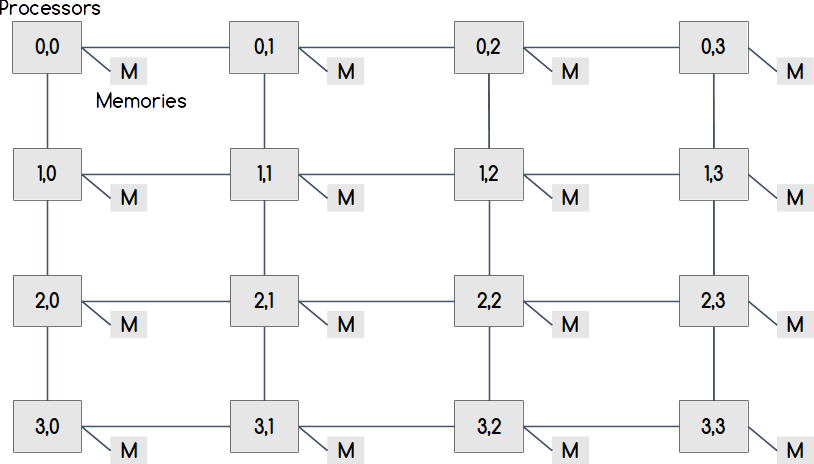
\includegraphics[width=0.7\linewidth]{meshconnected.png}
  \centering
  \caption{A mesh-connected distributed global memory system with 16 processors~\cite{dynamicPageMigration}.}
  \label{fig:mesh}
\end{figure}
\chapter{Concept and System Architecture}
This chapter will discuss the concept of our dynamic data migration scheme and will relate it to the state-of-the art discussed in Chapter 2. It will further explain the individual modules used in developing our scheme and will illustrate our system design.
\section{Concept}
The basic idea is to bring data and tasks close together in order to save execution time used in transferring data back and forth. In~\cite{dynamicPageMigration}, the authors have implemented a dynamic page migration scheme for a multiprocessor architecture which has mesh connection with a distributed-shared global memory as shown in figure \ref{fig:mesh}. Our architecture differs from theirs as we have tiles connected in a Network on Chip (NoC) as shown in figure \ref{fig:processor} whereas they have processors connected in a NoC.\\
\\
In~\cite{cacheDataPlacement1, cacheDataPlacement3, cacheDataPlacement4} the authors have done dynamic data placement for the last level cache (LLC) in order to reduce the distance between the data blocks and the core requesting it. We also want to bring data and the core requesting the data close together but we dynamically migrate data of the distributed shared tile local memory (TLM) instead of the LLC. In~\cite{threadPlacement4} the authors have used a thread scheduling mechanism which uses the performance monitoring unit (PMU) with hardware performance counters. For every thread the PMU maintain a summary vector which holds the signature of data regions accessed by a thread. In our scheme, we need to monitor the accesses made to the TLM of every tile in order to decide if migration is needed or not. The next section will explain how we monitor and categorize the accesses made to the TLM. \\
\begin{figure}
  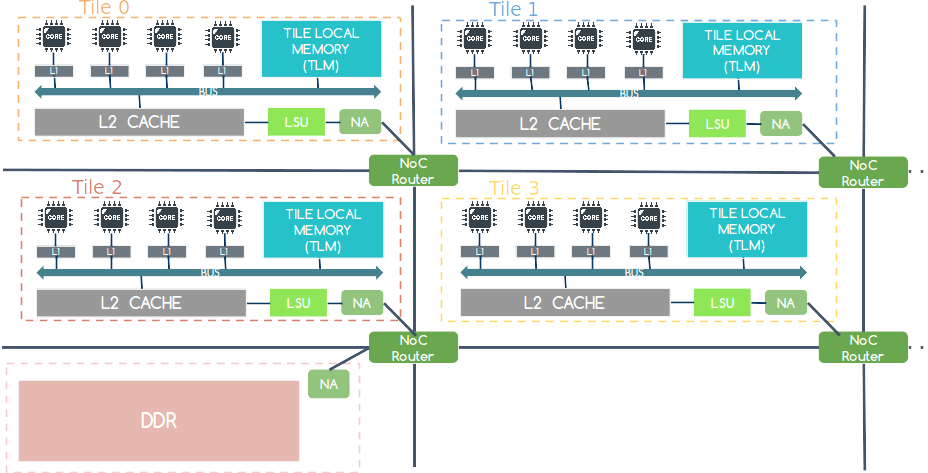
\includegraphics[width=\linewidth]{processor.png}
  \centering
  \caption{Our architecture.}
  \label{fig:processor}
\end{figure}
\subsection{Memory Accesses}
The Tile Local Memory (TLM) is a distributed-shared memory in the processor architecture. By distributed-shared we mean that it is distributed among all the tiles and can be accessed by cores placed remotely on neighboring or far away tiles. As mentioned in the previous chapter, figure \ref{fig:tile} depicts the inside of one tile. We have multiple such tiles in our processor as shown in figure \ref{fig:processor} hence the name multi-tile multi-core processor architecture. A TLM can have two kind of accesses to its data blocks:\\
\par
\textbf{Local TLM Accesses}: Figure \ref{fig:localaccesses} depicts different scenarios of when a request is considered a Local TLM Access. In tile 0 a core is accessing its local tile's memory which makes it a local TLM access. Also, in tile 1 a core is accessing data from a address of another tile's local memory but that data is cached in the L1 cache of the core requesting the data hence it becomes a Local TLM Access. Another scenario is a core in tile 1 accessing data from address of another tile's local memory but that data is cached in the L2 cache of the tile. It is again considered a Local TLM Access. In a Local TLM Access, the data transfer is happening over the bus inside the tile and there is no traffic going outside the tile through the network adapter. This takes less time as data is placed close to the core that uses it. \\
\begin{figure}
  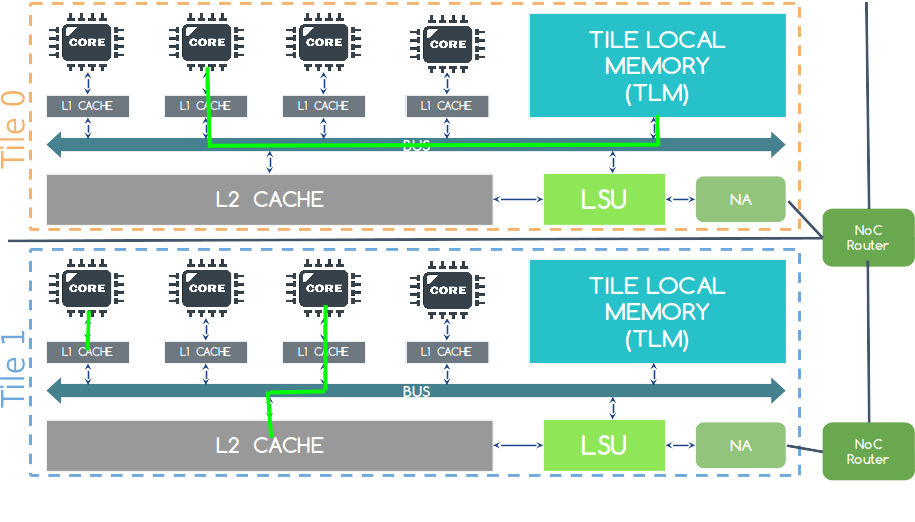
\includegraphics[width=\linewidth]{localaccesses.png}
  \centering
  \caption{A tile depicting local accesses to a TLM.}
  \label{fig:localaccesses}
\end{figure}
\par
\textbf{Remote TLM Accesses}: Figure \ref{fig:remoteaccesses} depicts a scenario where a core is accessing another tile's local memory (which is not cached in the L1 or L2 cache of the tile) which makes it a remote TLM access. In this scenario the data transfer is happening over the bus, through the LSU and network adapter and then the NoC Router routes it in the direction of the destination tile. This global access takes more time since data is placed far away from the core that uses it. 
\begin{figure}
  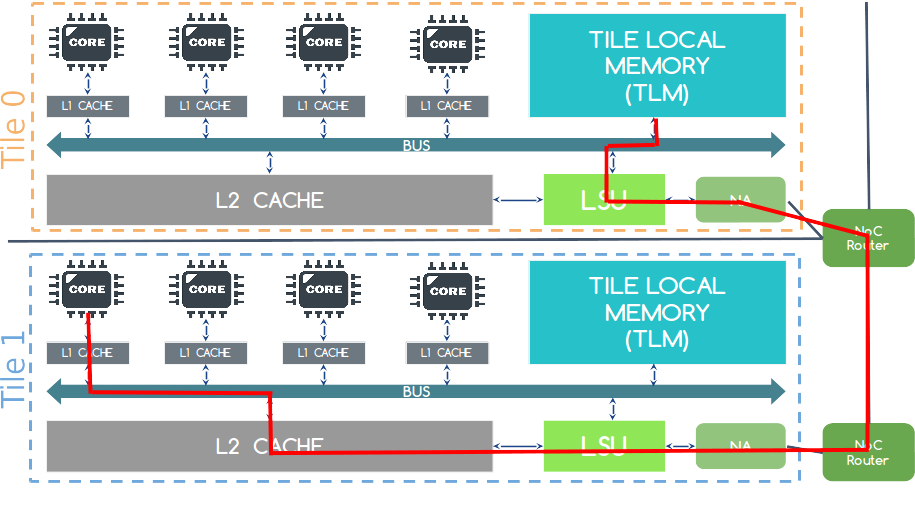
\includegraphics[width=\linewidth]{remoteaccesses.png}
  \centering
  \caption{A tile depicting remote accesses to a TLM.}
  \label{fig:remoteaccesses}
\end{figure}
\subsection{Goal}
We want to reduce the number of remote TLM accesses since it takes more time to fetch data from a TLM which is placed on another tile (as the request has to go on the bus through the network adapter and over the NoC Router in order to go to the other tile) and less time to fetch data which is on a core's own TLM.  
\section{System Design}
Figure~\ref{fig:overviewOfSolution} shows the overview of the modules involved in dynamic data migration scheme. Every cache module is connected to a Cache Stats Module. All these Cache Stats Modules and the TLM Modules report to the Central Stats Module at every given time interval (T$_{interval}$). The Cache Stats Module sends its number of local and remote accesses to the data blocks (TLM Blocks) whereas the TLM Modules send its free address space to the Central Stats Module. The Central Stats Module does evaluation of this data and triggers migration if needed. The migration command is passed by the Central Stats Module to the Cache Stats Module connected to the L2 Cache.\\
\begin{figure}
  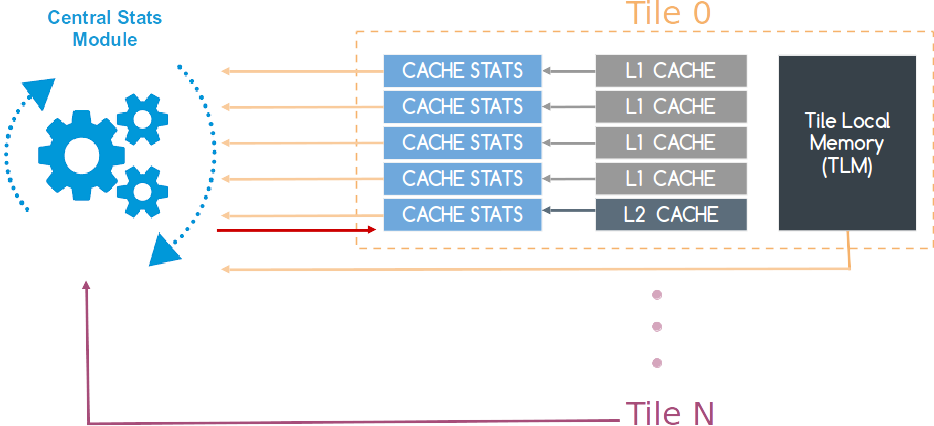
\includegraphics[width=\linewidth]{moduleconnections.png}
  \centering
  \caption{Overview and connections of the modules used.}
  \label{fig:overviewOfSolution}
\end{figure}
\\
Also, there is a Memory Management Unit which sits between the trace file and the Cores as shown in Figure \ref{fig:traceFile}. It contains the address translation for all the addresses from the DDR to the TLM. Every trace from the trace file first passes through the Memory Management Unit for address translation and then it is executed so that if there is a address translation entry present in the MMU for the particular address, the request accesses the data from the new location instead of the old one.\\ 
\begin{figure}[h!]
  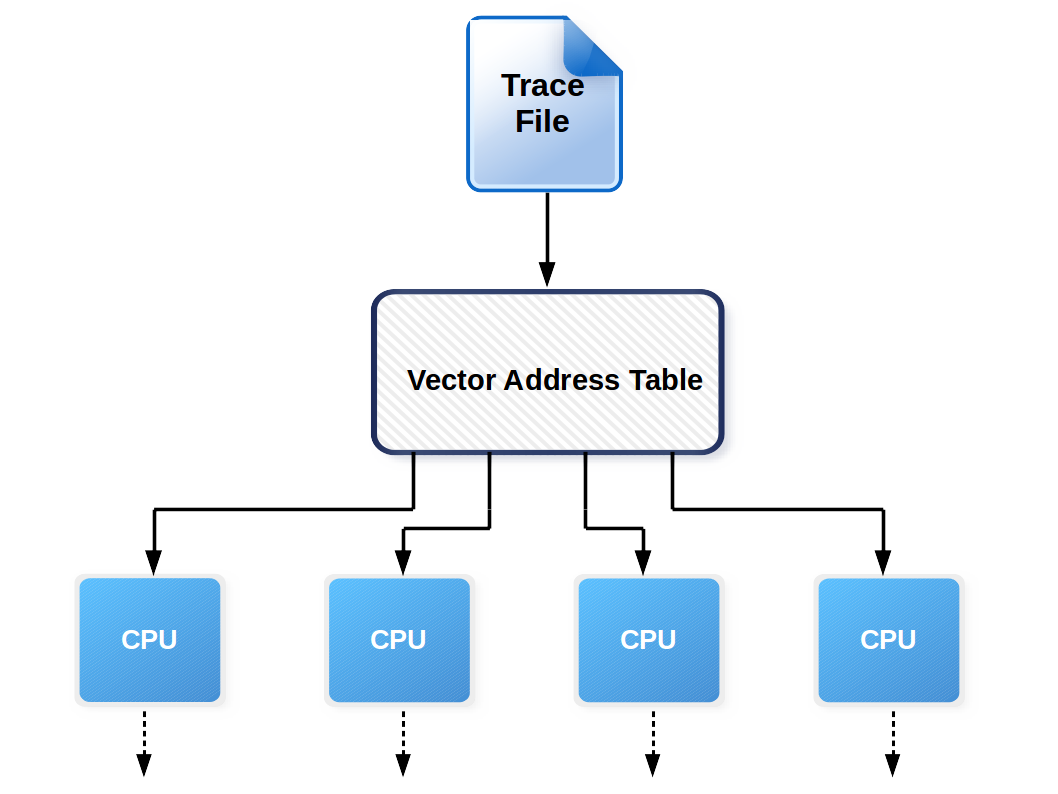
\includegraphics[width=0.7\linewidth]{traceFile.png}
  \centering
  \caption{Trace File and MMU}
  \label{fig:traceFile}
\end{figure}
\section{Modules Directly Used in the System for Implementing Thesis}
\subsection{Trace File}
As we use a trace based processor model, we first generate and save the traces in a file for different benchmarks using the gem5 simulator~\cite{gem5}. A trace file basically contains a set of read and write commands which is given to the simulator~\cite{akshay}. The commands are decoded by the processor (Read or Write) and are send to the rest of the modules for execution. A general trace in a trace file is depicted below:
\begin{table}[h!]
\begin{center}
 \begin{tabular}{c | c | c | c } 
 \textbf{Time-stamp} &  \textbf{Thread Number}  &  \textbf{RD/WR} &  \textbf{Address} \\ 
\end{tabular}
\end{center}
\end{table}
\begin{itemize}
  \item \textbf{Time-stamp}: The time in nanoseconds at which the trace is executed.
  \item \textbf{Thread Number}: The thread number which executed the trace.
  \item \textbf{RD/WR}: This value is set to 1 for a read command and 2 for a write command. 
  \item \textbf{Address}: The address to read data from or write data at.
\end{itemize}
Below are examples of traces for a read and write command followed by their explanations:
\begin{center}
 \begin{tabular}{c | c | c | c } 
 \textbf{2000} &  \textbf{2}  &  \textbf{1} &  \textbf{41012345} \\ 
\end{tabular}
\end{center}
At time 2000 ns, core 2 reads data from address 0x41012345.
\begin{center}
 \begin{tabular}{c | c | c | c } 
 \textbf{3500} &  \textbf{7}  &  \textbf{2} &  \textbf{41000FFF} \\ 
\end{tabular}
\end{center}
At time 3500 ns, core 7 writes data to address 0x41000FFF.\\
\\
It is important to note here that the traces of all the cores are present in one trace file. This means that all the cores access the same trace file as shown in figure~\ref{fig:traceFile}. Each core needs to decode and execute the traces which matches only with its core number.
\subsection{Memory Management Unit}
The Memory Management Unit (MMU) sits between the trace file and the cores as shown in Figure \ref{fig:traceFile}. This unit is basically a vector address table which contains the address translation of all the addresses from the DDR to the TLM. At start all TLM's are empty which means every instruction has to access data from the DDR. The memory management unit's is updated if a migration triggered by the Central Stats Module takes place.
Below is a example of a vector address table with two entries.\\
\begin{center}
 \begin{tabular}{c | c } 
 \hline
 \textbf{Original} &  \textbf{New}  \\
 \hline
 \rule{0pt}{4ex}     \ \ \ \ \ \ 31012345 \ \ \ \ \ \ &   \ \ \ \ \ \ 44012345 \ \ \ \ \ \ \\ 
  \ \ \ \ \ \ 41000FFF \ \  \ \ \ \ &  \ \ \ \ \ \ 40000FFF \ \ \ \ \ \ \\ 
\end{tabular}
\end{center}
The values signify that the data at address 0x31012345 has been migrated to the address 0x44012345. Similarly, the data at address 0x41000FFF has been migrated to the address 0x40000FFF.
\subsection{Cache Stats Module}
The Cache Stats Module is depicted in figure~\ref{fig:overviewOfSolution}. It is connected to the L1 and L2 Caches and is continuously getting updates from them regarding cache hits and misses per cache line. This module is responsible for calculating the cache hits and misses per TLM Block which can vary in size from 1 cache line to multiple cache lines. It also calculates the number of local and remote accesses for every TLM Block. Cache Stats Module also plays a important role in carrying out the data migration command as the migration command has to go through this module. 
\subsection{Tile Local Memory Module}
This is the Tile's Local Memory and has been explained in detail in chapter 2. This module has the functionality to observe itself and calculate whether it is empty or has free space. If it has free space then it can find the starting and ending address of all the free spaces. 
\subsection{Central Stats Module}
This is the main central module to whom all the Cache Stats Modules and TLM Modules report to every given time interval (T$_{interval}$). This module is responsible for evaluating the data and determining whether migration(s) shall take place or not.
\chapter{Implementation}
This chapter will talk about the technologies used to develop the system. It will also discuss the detailed approach of developing the dynamic data migration scheme. We further talk in detail about how the parameters responsible for data migration are calculated and the limitations that exists in the simulator. \\
\section{Language and Tools}
\subsection{SystemC}
The simulator is modeled using SystemC~\cite{systemc}. SystemC is basically classified as a set of C++ classes rather than a language. It provides an event-driven simulation interface which enables the user to simulate concurrent processes and do system level modeling. One of the major concept used in SystemC is \textit{Transaction Level Modeling (TLM)}. In TLM the details of communication among modules are separated from the details of the implementation of the functional modules~\cite{tlm}. It provides defined rules for how different modules (namely known as \textit{Initiator} and \textit{Target}) should communicate with each other. \\
\\
The simulator is modeled using the TLM-2.0 standard protocol~\cite{systemc}. This standard supports two types of non-blocking communication i.e \textit{TLM-2.0 Two Phase Protocol} and \textit{TLM-2.0 Four Phase Protocol}~\cite{akshay}. Non-blocking communication means that function implementations never wait for the response from the target.
\subsection{Synopsys Platform Architect}
The simulator is powered by Synopsys Platform Architect Tool~\cite{synopsys}. Synopsys Platform Architect is a SystemC TLM standards-based graphical environment which can be used as a alternative to a SystemC top level module for binding the individual modules. With this tool the individual modules just need to be imported and connected together graphically. This makes the connection of multiple modules with multiple initiator-target socket pairs easier to design and debug.\\
\\ Figure~\ref{fig:insidetile} represents the internal view of the tile in Synopsys Platform Architect Tool. It contains four cores, each core having its own private L1 cache and a TLM. The L1 caches are connected together by a bus. Figure~\ref{fig:processorsynopsys} illustrates how the tiles are connected together in the processor architecture. The detailed explanation of the architecture design has been given in Chapter 3. It can be seen from figure~\ref{fig:insidetile} and figure~\ref{fig:processorsynopsys} that the graphical view of the tool helps in visualizing complex systems and makes the design phase easier which in turn makes testing and debugging easier.
\begin{figure}
  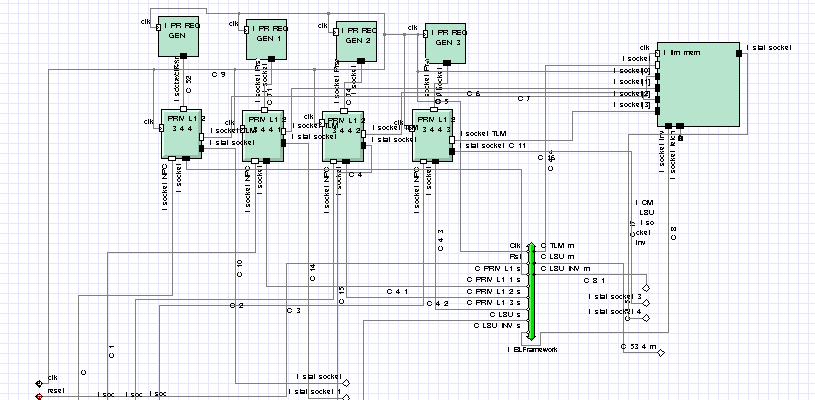
\includegraphics[width=\linewidth]{insidetile.png}
  \centering
  \caption{Intra-Tile Design View in Synopsys Platform Architect}
  \label{fig:insidetile}
\end{figure}
\begin{figure}
  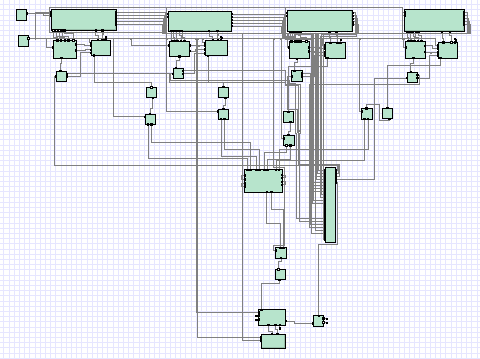
\includegraphics[width=\linewidth]{processorsynopsys.png}
  \centering
  \caption{Inter-Tile Design View in Synopsys Platform Architect}
  \label{fig:processorsynopsys}
\end{figure}
\section{Dynamic Data Migration Process Mechanism}
Figure \ref{fig:approachOfSolution} shows the messages exchanged between the Cache Stats Module, TLM Module and Central Stats Module. At every given time interval (T$_{interval}$) the Cache Stats Module sends the number of local and remote accesses of all the TLM blocks to the Central Stats Module and the TLM Module sends its free address space to the Central Stats Module. The TLM block size is equal to a variable number of cache lines that is determined at compile time by the user. The Central Stats module then evaluates this received data and sends a migrate command to the L2 Cache Stats module if the need arises. \\
\\
The next subsections will explain how the messages exchanged between the modules are calculated. 
\begin{figure}
  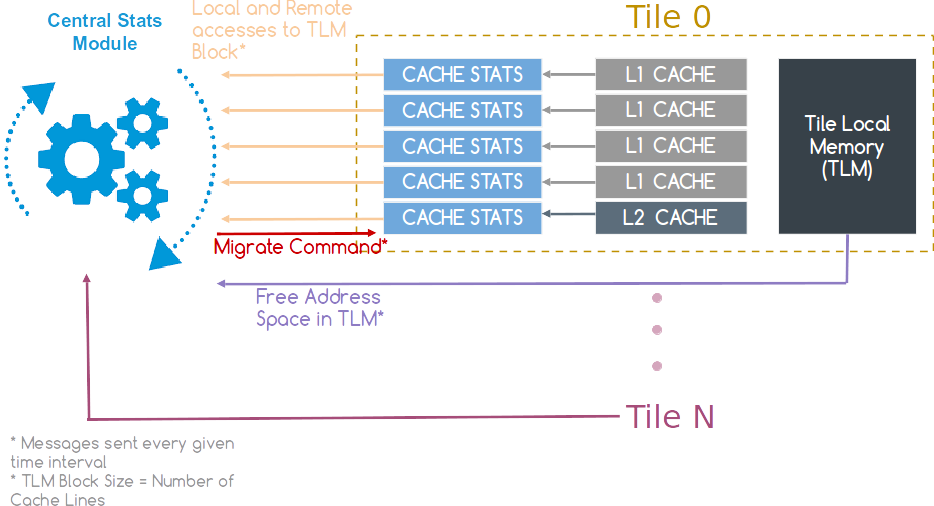
\includegraphics[width=\linewidth]{approachOfSolution1.png}
  \centering
  \caption{Messages exchanged between the Cache Stats, TLM and Central Stats Modules.}
  \label{fig:approachOfSolution}
\end{figure}
\subsection{Triggering Migrations}
\subsubsection{Which TLM Block to Migrate and Tile to Migrate it to?}
Figure \ref{fig:tiletomigrate} shows how the tile to migrate a certain TLM block is determined in the Central Stats Module. For every TLM Block the local and remote accesses are sent by the Cache Stats Module to the Central Stats Module. For every TLM Block, first it is checked whether it is a DDR address or a TLM address. If it is a DDR address the tile with the highest number if local accesses is found and that is the tile to migrate the DDR address (TLM Block) to. This is because a DDR address can be a remote access only when it is placed in the DDR, else it is cached in and is always a local access. If the address is not a DDR address then the tile with the maximum number of remote accesses is found. These number of local accesses are compared to the local accesses for the TLM Block. If these remote accesses are greater then the local accesses then it signifies that it has to be migrated to this tile. \\
\begin{figure}
  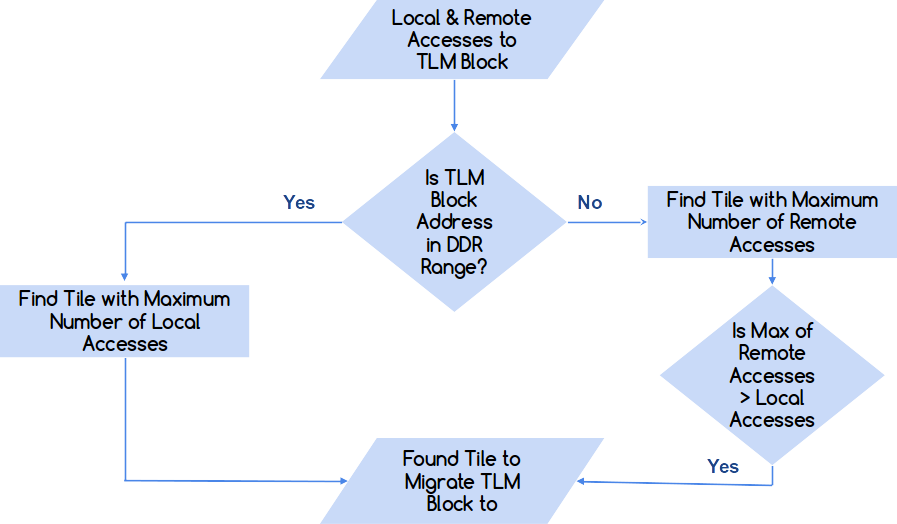
\includegraphics[width=\linewidth]{tiletomigrate.png}
  \centering
  \caption{Process to determine the TLM Block to migrate and the tile to migrate the TLM Block to.}
  \label{fig:tiletomigrate}
\end{figure}
\subsubsection{When to Trigger Migrations?}
Figure \ref{fig:tlm_stats flowchart} shows the algorithm for determining when migration shall take place. After we know the tile to which a specific TLM block shall be migrated, it is determined whether there is free space in that tile's local memory. If there is free space, a migration command is send to L2 Cache Stats module. \\
\\
However, if there is no free space in the TLM, then the block with the least number of local accesses in the TLM is identified and this number of local accesses is compared with the number of remote accesses of the TLM block which is to be migrated. If the number of remote accesses of the TLM block to be migrated is higher than this number of local accesses the data between the two memory locations is swapped which means a migration command is send to the L2 Cache Stats module for the TLM block in the TLM which is full i.e the TLM block in the TLM which is full is copied to a buffer in order to make space for the incoming TLM block. Now with free space in the TLM a migration command is send to the L2 Cache Stats module of the incoming TLM block. Once this migration is completed the value in the buffer is copied into this memory location. If the remote accesses of the TLM block to be migrated are less than the minimum local accesses in the TLM then the migration is flushed.\\
\\
In case all the local accesses to a TLM are equal and a minimum cannot be found then at random a TLM Block is picked and the local accesses are compared with the migrating TLM Block's remote accesses. If the former is smaller than the latter, the TLM block is swapped with the incoming TLM block. Otherwise the migration is flushed.\\
\subsubsection{Migrate Command}
The migrate command is split into two commands in the Cache Stats module; first reading data from the location from where data has to be migrated and then writing data at the new location to which the migration is taking place. Once, the data is read a invalidation command is sent to all L1 and L2 caches for that TLM Block and once the data is written the vector address table in the memory management unit is updated. If a request is made to a address whose migration is in transition i.e data has been read from that address and invalidations have been sent to L1 and L2 caches but it has not been written to the new address yet, that request is pushed to a priority queue and is completed once the migration is complete and the vector address table is updated.\\
\begin{figure}
  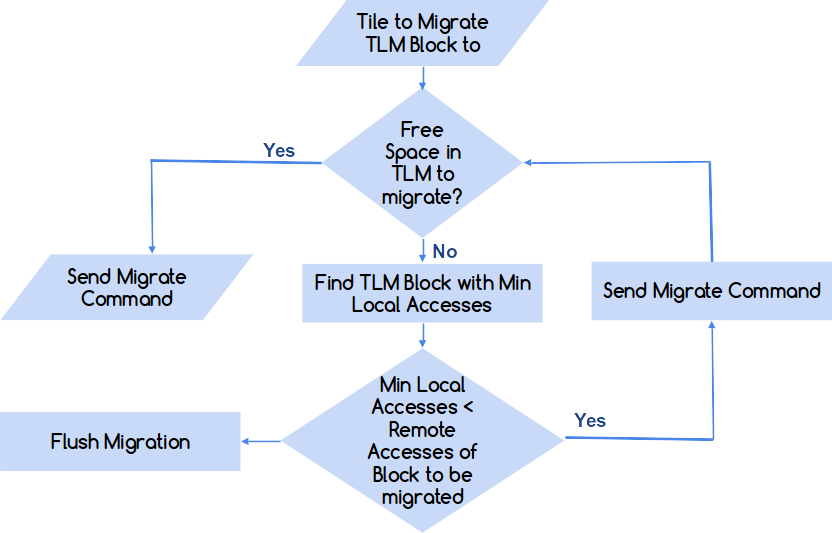
\includegraphics[width=\linewidth]{tlmstats.png}
  \centering
  \caption{Triggering Migration Commands}
  \label{fig:tlm_stats flowchart}
\end{figure}
\subsection{Local and Remote Accesses to a TLM Block}
Figure \ref{fig:remoteLocalAccess} shows the calculation behind the metric of local access and remote access to a TLM Block in the Cache Stats module. We compare the TLM number which is being accessed by a trace with the current tile number (the tile where the cache stats module is placed). If the two values are equal it means it is a request to the TLM of the same tile which signifies it is a local access. If the two values are different it implies it is a request for another tile's TLM and we check whether there is a L1 cache hit or miss. If there is a L1 cache hit, it is a local access. However, if it is a L1 cache miss then we check whether it is a L2 cache hit or miss. If it is a hit then it a local access but if it is a miss then we have a remote access. \\
\begin{figure}
  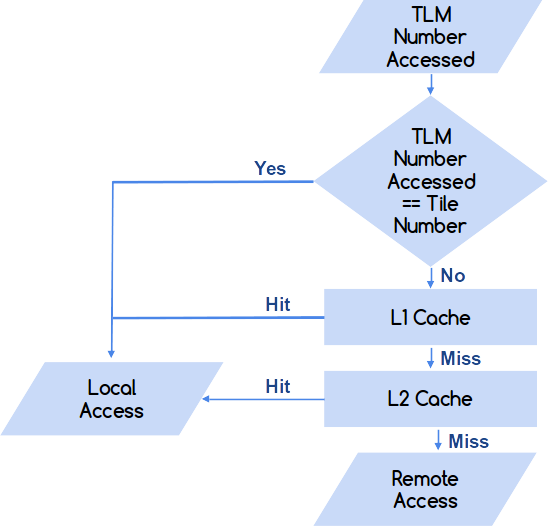
\includegraphics[width=0.6\linewidth]{localandremote.png}
  \centering
  \caption{Flowchart illustrating how to determine a local and remote TLM access.}
  \label{fig:remoteLocalAccess}
\end{figure}

\subsection{Free Address Space in TLM}
Figure \ref{fig:freeSpaceTLM} shows how we find the free address space in the TLM Module. For calculating the free address space in the TLM we can have three scenarios. 
\begin{figure}
  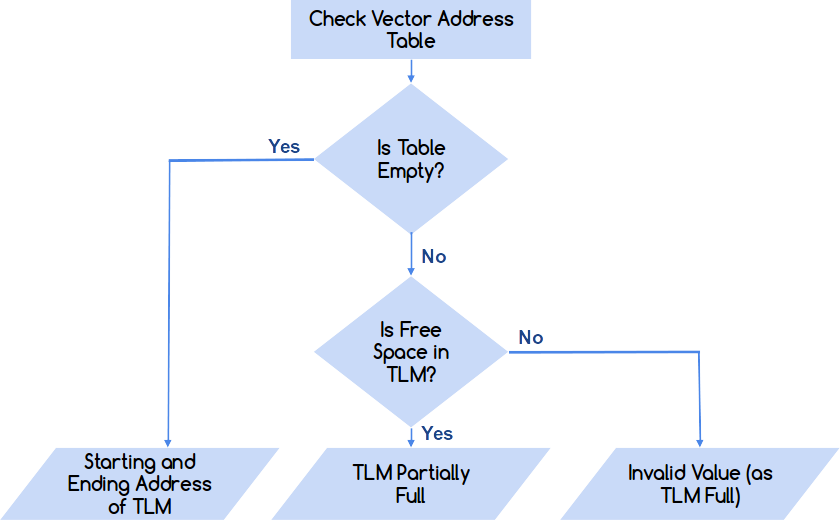
\includegraphics[width=\linewidth]{freespace.png}
  \centering
  \caption{Flowchart depicting how the free address space in the TLM is calculated.}
  \label{fig:freeSpaceTLM}
\end{figure}
\begin{enumerate}
  \item TLM Empty 
  \item TLM Partially Full
  \item TLM Full
\end{enumerate}
\subsubsection{TLM Empty}
If the vector address table in the memory management unit is empty then we know straightaway that the TLM is empty. In that scenario, the starting and ending address of the TLM address space are sent to the Central Stats Module.\\ 
\subsubsection{TLM Partially Full}
If the vector address table in the memory management unit is not empty we iterate over the table and extract the addresses belonging to the current tile's TLM. After we have these addresses we analyze them and determine the free address space in the TLM. The starting and ending address of one free space block is send to the Central Stats Module.\\
\begin{figure}
  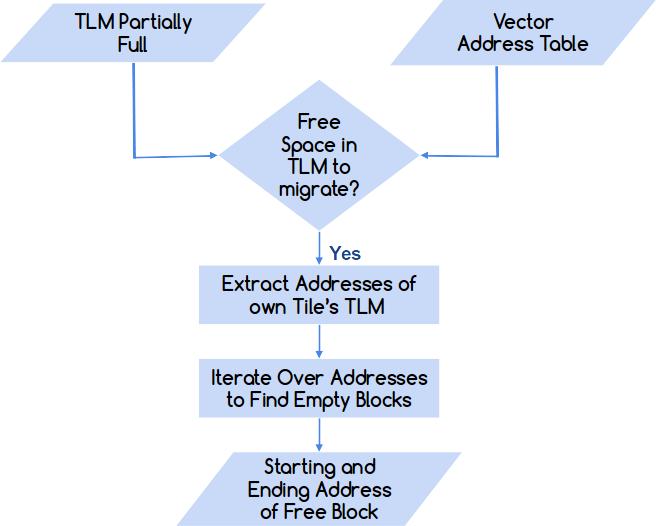
\includegraphics[width=0.7\linewidth]{tlmpartiallyempty.png}
  \centering
  \caption{Flowchart showing how the free address space in TLM is calculated if the TLM is partially full.}
  \label{fig:freeSpaceTLM}
\end{figure}
\subsubsection{TLM Full}
In this case also the vector address table in the memory management unit is not empty. We extract the addresses belonging to the current tile's TLM and if there is no space in the TLM we inform the Central Stats Module this by sending a invalid value.\\
\section{Usability Improvement}
In the simulator we have now given an option to turn dynamic data migration on and off by setting a parameter from the command line or from within the tool Synopsys. It makes the result gathering phase easier and quicker. Also, since the TLM Block size and the time interval (T$_{interval}$) are variable and can be changed by the user; the change in performance or execution time by varying these two parameters can be analyzed.
\section{Limitations}
Adding the dynamic data migration support to the simulator increases the real time of the simulation due to the high number of computations that are being done to determine migrations. \\
\\
In the simulator the main modules added because of the dynamic data migration scheme are:
\begin{itemize}
  \item Twenty-one Cache Stats modules
  \item One Central Stats module 
  \item One Memory Management Unit
\end{itemize}
The memory requirements increases due to these modules. 

\chapter{Experimental Setup}
This chapter will lay out the programs that assisted in running the simulations. Moreover, it will also illustrate the specifications of the machine that were utilized to run the experiments.
\section{Configuration of Component Modules}
This section illustrates the configuration properties of the modules in the simulations used for the result gathering.
\subsection{Configuration of TLM}
Table~\ref{table:Size} shows the configuration of the tile local memory used in the simulations. The address bits are 24 which means the address of each TLM spans from the values shown in table~\ref{table:addressTLM}
\begin{table}[h!]
\begin{center}
 \begin{tabular}{|| c | c ||} 
 \hline
 \ \textbf{Paramater} & \textbf{Value}  \\ [0.5 ex] 
 \hline\hline
 \ \ \ \ \ \ \ \ Address Bits \ \ \ \ \ \ \ \ & \ \ \ \ \ \ \ \ 24 \ \ \ \ \ \ \ \ \\ 
 \hline
 \ \ \ \ \ \ \ \ Data Width\ \ \ \ \ \ \ \ & \ \ \ \ \ \ \ \ 8 \ \ \ \ \ \ \ \ \\
 \hline
 \ \ \ \ \ \ \ \ Size in MB \ \ \ \ \ \ \ \ & \ \ \ \ \ \ \ \ 16 \ \ \ \ \ \ \ \  \\
 \hline
\end{tabular}
 \caption{TLM Configuration}
 \label{table:Size}
\end{center}
\end{table}

\begin{table}[h!]
\begin{center}
 \begin{tabular}{|| c | c ||} 
 \hline
 \ \textbf{TLM Number} & \textbf{Address Range}  \\ [0.5 ex] 
 \hline\hline
 \ \ \ \ \ \ \ \ TLM 0 \ \ \ \ \ \ \ \ & \ \ \ \ \ \ \ \ 0x40000000 - 0x40FFFFFF \ \ \ \ \ \ \ \ \\ 
 \hline
 \ \ \ \ \ \ \ \ TLM 1\ \ \ \ \ \ \ \ & \ \ \ \ \ \ \ \ 0x41000000 - 0x41FFFFFF  \ \ \ \ \ \ \ \ \\
 \hline
 \ \ \ \ \ \ \ \ TLM 2 \ \ \ \ \ \ \ \ & \ \ \ \ \ \ \ \ 0x42000000 - 0x42FFFFFF  \ \ \ \ \ \ \ \  \\
 \hline
  \ \ \ \ \ \ \ \ TLM 3 \ \ \ \ \ \ \ \ & \ \ \ \ \ \ \ \ 0x43000000 - 0x43FFFFFF  \ \ \ \ \ \ \ \  \\
  \hline
\end{tabular}
 \caption{Address Range of each TLM}
 \label{table:addressTLM}
\end{center}
\end{table}

\subsection{Configuration of Data Caches}
Table 5.3 shows the configuration of the data caches used for the simulations
\begin{table}[h!]
\begin{center}
 \begin{tabular}{|| c | c ||} 
 \hline
 \ \textbf{Parameter} & \textbf{Value}  \\ [0.5 ex] 
 \hline\hline
  Data Cache Line Size in Number of Words &  4  \\
  \hline
  Number of Data Cache Ways &  2  \\
  \hline
  Data Cache Replacement Policy  & Least Recently Replaced  \\ 
 \hline
  Write Policy  &  Write-through  \\
  \hline
\end{tabular}
 \caption{Data Cache Configuration}
 \label{table:properties}
\end{center}
\end{table}

\subsection{Configuration of DDR}
Table 5.4 shows the configuration of the DDR used for the simulations
\begin{table}[h!]
\begin{center}
 \begin{tabular}{|| c | c ||} 
 \hline
 \ \textbf{Paramater} & \textbf{Value}  \\ [0.5 ex] 
 \hline\hline
 \ \ \ \ \ \ \ \ Address Bits \ \ \ \ \ \ \ \ & \ \ \ \ \ \ \ \ 64 \ \ \ \ \ \ \ \ \\ 
 \hline
 \ \ \ \ \ \ \ \ Data Width\ \ \ \ \ \ \ \ & \ \ \ \ \ \ \ \ 32 \ \ \ \ \ \ \ \ \\
 \hline
 \ \ \ \ \ \ \ \ Size in GB \ \ \ \ \ \ \ \ & \ \ \ \ \ \ \ \ 1 \ \ \ \ \ \ \ \  \\
 \hline
 \ \ \ \ \ \ \ \ Address Range \ \ \ \ \ \ \ \ & \ \ \ \ \ \ \ \ 0x00000000 - 0x3FFFFFFF \ \ \ \ \ \ \ \  \\
  \hline
\end{tabular}
 \caption{DDR Configuration}
 \label{table:DDR}
\end{center}
\end{table}
\section{The Gem5 Simulator}
The Gem5 simulator~\cite{gem5},~\cite{akshay} is a modular event driven platform for computer system architecture. It is used for research and can be used to simulate different computer architectures. It can be operated in two modes:
\begin{itemize}
\item System Call Emulation (SE) Mode: In this mode, the user only needs to specify the binary file to be simulated.
\item Full System (FS) Mode: In this mode, the benchmarks are booted on a dedicated operating system with proper scheduling support. 
\end{itemize}
 We use the Gem5 in Full System simulator mode in order to generate the trace file for our simulations. This mode results in higher accuracy than the SE mode.
\section{Benchmarks}
To evaluate the effectiveness of dynamic data migration, we need to choose some parallel benchmarks to run on the simulator. These benchmarks have to be executed with the Gem5 simulator in-order to have the memory access traces in a trace file which is then given as input to the simulator. For all our simulations, we make use of workloads from the PARSEC Benchmark Suite~\cite{lispaper},~\cite{trace}. We choose three parallel workloads covering three application domains and generate their trace files. The three workloads are: 
\begin{itemize}
\item Blackscholes (Financial Analysis)
\item Swaptions (Financial Analysis)
\item Canneal (Engineering)
\end{itemize}
\section{Writing Shell Script}
A shell script for running the migration command is written so that multiple simulations can run in parallel without the need to recompile the simulator. The maximum number of parallel simulations that we could run was four. This saved us considerable time in gathering results. 
\section{\textit{Nice} Command}
The script is run with \textit{nice} command~\cite{nice} which runs the simulation with a different priority then the usual. We ran the simulations with a increased priority of nine.
\section{Output Files}
The output of the simulation is saved in different text files. The files important for this thesis are:
\begin{itemize}
\item Screen Log File
\item Time Log File
\end{itemize}
\subsection{Screen Log File}
The screen log file gives the virtual processing time (in nano seconds) of each processor and also of the entire system. It also gives the real time, the user time and the system time of running the simulations in minutes and seconds. Further it gives the total number of remote reads and remote writes of the simulation run and some other parameters and queue sizes that are not relevant for this thesis.\\
\subsection{Time Log File}
The time log file consists of the breakdown of the virtual time (in nano seconds) that each processor took executing instructions on different tiles and on the individual components/modules like TLM, L1-Cache, NPC, NoC, Bus etc.
\section{System Specifications}
The simulations were run on a core i5 Intel processor. The operating system is Ubuntu 16.04.4 LTS and th PC has a RAM of 15 GB.
\chapter{Evaluation}
This chapter illustrates the results gathered from the simulator. It gives the comparison of the execution time of the simulator with data migration on against the first touch and no data placement. It also shows the effect on execution time with varying block sizes and time intervals.
\section{Dynamic Data Migration vs First Touch and No Data Placement}
In this section the outcome of the simulation is analyzed and the performance of every benchmark is compared. Basically the execution time when dynamic data migration is turned on and data placement is none (i.e everything is in the DDR) is compared with the execution time of data placed via first touch and with no data placement with dynamic data migration turned off for the three benchmarks (trace files introduced in Section 5.3). Table 6.1 shows the execution times for the three benchmarks. The block size is one cache line and the time interval is 1000 nsec. The table is also illustrated as a bar graph in figure \ref{fig:Bla_cann_Swap_BS_1_T_1000.png}. For backscholes there has been a 20\% improvement in the execution time when DDM is ON versus DDM-OFF whereas for canneal the improvement is 6\%. Fow swaptions we don't see any improvement in the execution time because very few migrations were triggered by the system.\\
\\
\begin{table}[h!]
\begin{center}
 \begin{tabular}{|| c | c | c | c||} 
 \hline
 \ \textbf{Benchmark} & \textbf{DDM OFF - FT}  & \textbf{DDM ON - NONE}  & \textbf{DDM OFF - NONE}\\ [0.5 ex] 
 \hline\hline
  Blackscholes   &   3 762 137   &   16 954 398	    &  21 157 717 \\ 
 \hline
   Canneal  	&   3 498 151    &   38672029   	&   41 357 304   \\
 \hline
    Swaptions   &   9 836 531     &   133 304 375 	&   133 393 869   \\
 \hline
\end{tabular}
 \caption{Execution times in (\textbf{in nano-seconds}). The block size is one cache line and the time interval is 1000 nsec}
 \label{table:ExecTimes1}
\end{center}
\end{table}
\\
Table 6.2 shows the execution times for the three benchmarks when the block size is four cache lines and the time interval is 500 nsec. The table is also illustrated as a bar graph in figure \ref{fig:Bla_cann_Swap_BS_4_T_500.png}. For backscholes there has been a 46\% improvement in the execution time when DDM is ON versus DDM-OFF whereas for canneal the improvement is 47\%. Fow swaptions the improvement is 8\%.
\begin{table}[h!]
\begin{center}
 \begin{tabular}{|| c | c | c | c||} 
 \hline
 \ \textbf{Benchmark} & \textbf{DDM OFF - FT}  & \textbf{DDM ON - NONE}  & \textbf{DDM OFF - NONE}\\ [0.5 ex] 
 \hline\hline
  Blackscholes   &   3 762 137   &   11 343 765	    &  21 157 717 \\ 
 \hline
   Canneal  	&   3 498 151    &   21 753 905   	&   41 357 304   \\
 \hline
    Swaptions   &   9 836 531     &   122 806 943 	&   133 393 869   \\
 \hline
\end{tabular}
 \caption{Execution times in (\textbf{in nano-seconds}). The block size is four cache lines and the time interval is 500 nsec}
 \label{table:ExecTimes2}
\end{center}
\end{table}

\begin{figure}
  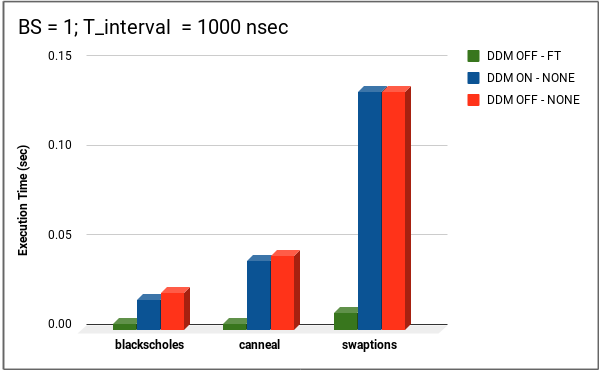
\includegraphics[width=\linewidth]{Bla_cann_Swap_BS_1_T_1000.png}
  \centering
  \caption{Bar Chart comparing the execution times for all the three trace files}
  \label{fig:Bla_cann_Swap_BS_1_T_1000.png}
\end{figure}

\begin{figure}
  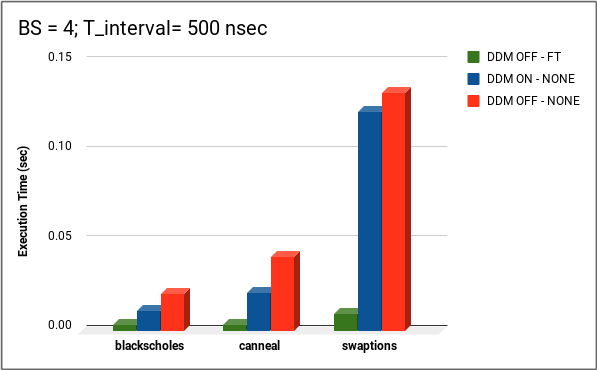
\includegraphics[width=\linewidth]{Bla_cann_Swap_BS_4_T_500.png}
  \centering
  \caption{Bar Chart comparing the execution times for all the three trace files}
  \label{fig:Bla_cann_Swap_BS_4_T_500.png}
\end{figure}

\section{Blackscholes}
Table 6.3 shows the execution times for varying time intervals and block sizes for blackscholes. The results are also illustrated in figure \ref{fig:Blacksc_var_bs_t.png}. It can be seen in the figure that we get the best performance when our block size is large (16 cache lines) and our time interval is small (200 nsec). The graphs saturates for all block sizes at larger time intervals since very few migrations get triggered. 

\begin{table}[h!]
\begin{center}
 \begin{tabular}{|| c | c | c | c| c | c | c | c||} 
 \hline
 \ \textbf{BS} & \textbf{200ns}  & \textbf{500ns}  & \textbf{1000ns} & \textbf{10000ns} & \textbf{20000ns} & \textbf{50000ns} & \textbf{100000ns}\\ [0.5 ex] 
 \hline\hline
   1 & 14 425 857  & 15 268 789 &  16 954 398 & 19 292 264 & 20 803 545 & 20 850 647 &  211 57 717\\ 
 \hline
   2 & 13 651 220 & 12 785 944 & 14 249 915 & 20 017 107 & 20 448 252 & 20 904 470 & 21 041 269\\
 \hline
   4 & 8 631 100 & 11 343 765 & 14 782 794 & 20 981 453 & 19 811 044 & 20 896 761 & 20 876 219\\
 \hline
   8 & 9 872 980 & 9 092 486 & 12 989 437 & 19 478 459 & 18 086 612 & 17 918 226 & 19 444 638\\
  \hline
   16 & 4 764 657 & 9 092 486 & 12 989 437 & 19 478 459 & 18 086 612 & 17 918 226 & 19 444 638\\
    \hline
\end{tabular}
 \caption{Blackscholes: execution times in (\textbf{in nano-seconds}) for varying block sizes and time intervals}
 \label{table:ExecTimes2}
\end{center}
\end{table}

\begin{figure}
  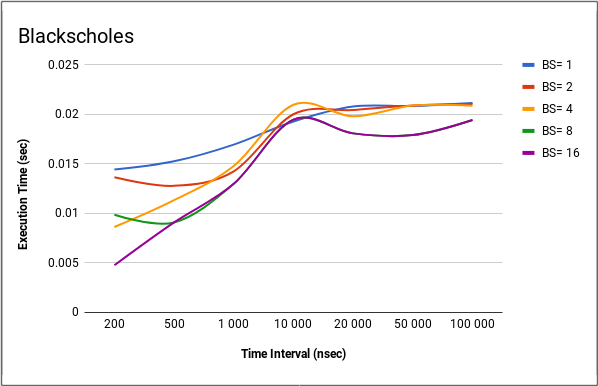
\includegraphics[width=\linewidth]{Blacksc_var_bs_t.png}
  \centering
  \caption{Graph showing how the execution time varies with varying block sizes and time intervals for Blackscholes}
  \label{fig:Blacksc_var_bs_t.png}
\end{figure}

\section{Canneal}
Table 6.4 shows the execution times for varying time intervals and block sizes for canneal. The results are also illustrated in figure \ref{fig:cann_var_bs_t.png}. It can be seen in the figure that we get the best performance when our block size is 4 cache lines and our time interval is 500 nsec. The graphs saturates for all block sizes at larger time intervals since very few migrations get triggered. 

\begin{table}[h!]
\begin{center}
 \begin{tabular}{|| c | c | c| c | c | c | c||} 
 \hline
 \ \textbf{BS}  & \textbf{500ns}  & \textbf{1 000ns} & \textbf{10 000ns} & \textbf{20 000ns} & \textbf{50 000ns} & \textbf{100 000ns}\\ [0.5 ex] 
 \hline\hline
   1 & 34 615 158 &  38 672 029 & 41 357 391 & 41 357 355 & 41 354 429 &  41 350 129 \\ 
 \hline
   2 & 28 026 014 & 35 936 653 & 41 357 748 & 41 357 458 & 41 357 304 & 41 357 304 \\
 \hline
   4 & 21 753 905 & 35 370 422 & 41 052 980 & 41 357 365 & 41 357 304 & 41 357 304 \\
 \hline
   8 & 31 874 829 & 31 874 829 & 39 580 017 & 41 357 395 & 41 357 304 & 41 357 304 \\
  \hline
   16 & 31 874 829 & 31 874 829 & 39 580 017 & 41 357 395 & 41 357 304 & 41 357 304 \\
    \hline
\end{tabular}
 \caption{Canneal: execution times in (\textbf{in nano-seconds}) for varying block sizes and time intervals}
 \label{table:ExecTimes2}
\end{center}
\end{table}

\begin{figure}
  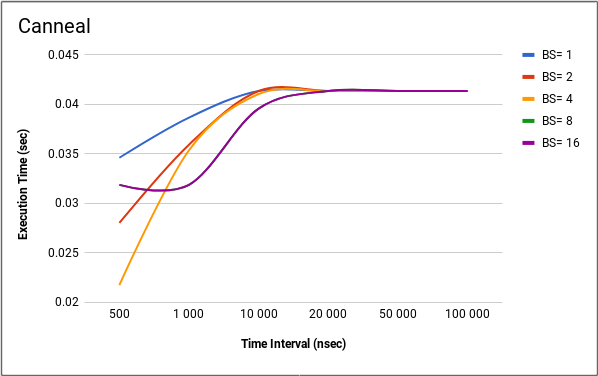
\includegraphics[width=\linewidth]{cann_var_bs_t.png}
  \centering
  \caption{Graph showing how the execution time varies with varying block sizes and time intervals for Canneal}
  \label{fig:cann_var_bs_t.png}
\end{figure}

\section{Swaptions}
Table 6.5 shows the execution times for varying time intervals and block sizes for swaptions. The results are also illustrated in figure \ref{fig:Swapt_var_bs_t.png}. It can be seen in the figure that we get the best performance when our block size is 4 cache lines and our time interval is 500 nsec. The graphs saturates for all block sizes at larger time intervals since very few migrations get triggered. 

\begin{table}[h!]
\begin{center}
 \begin{tabular}{|| c | c | c| c | c | c | c||} 
 \hline
 \ \textbf{BS}  & \textbf{500ns}  & \textbf{1 000ns} & \textbf{10 000ns} & \textbf{20 000ns} & \textbf{50 000ns} & \textbf{100 000ns}\\ [0.5 ex] 
 \hline\hline
   1 & 129 737 475 &  133 304 375 & 133 398 867 & 133 393 869 & 133 328 254 &  133 393 869 \\ 
 \hline
   2 & 123 952 879 & 132 674 834 & 133 335 126 & 133 393 895 & 133 393 869 & 133 393 869 \\
 \hline
   4 & 122 806 943 & 129 576 123 & 133 395 549 & 133 393 871 & 133 393 869 & 133 393 869 \\
 \hline
\end{tabular}
 \caption{Swaptions: execution times in (\textbf{in nano-seconds}) for varying block sizes and time intervals}
 \label{table:ExecTimes3}
\end{center}
\end{table}

\begin{figure}
  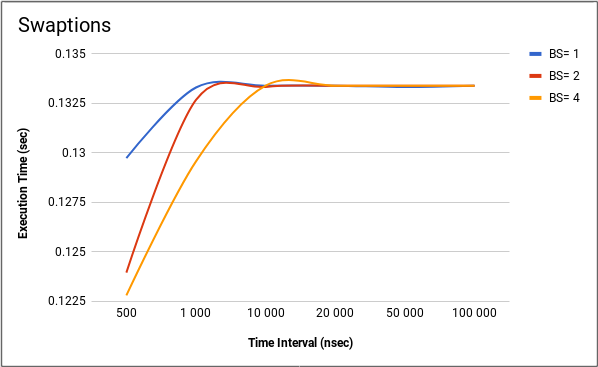
\includegraphics[width=\linewidth]{Swapt_var_bs_t.png}
  \centering
  \caption{Graph showing how the execution time varies with varying block sizes and time intervals for Swaptions}
  \label{fig:Swapt_var_bs_t.png}
\end{figure}

\section{Comparison of First Touch DDM ON with First Touch DDM OFF}
This section gives a comparison of the execution time when data is placed on the TLM using first touch policy and then the simulation is run first with dynamic migration turned on and then without dynamic data migration. As can be seen in figure \ref{fig:FT_DDM_ON_OFF_BLACK.png} the performance improves by 6\% when dynamic data migration is turned on. 

\begin{figure}
  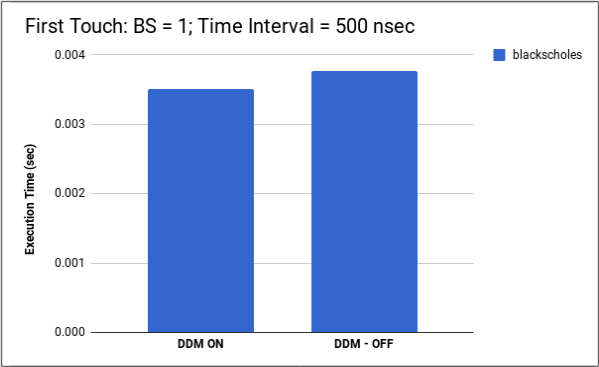
\includegraphics[width=\linewidth]{FT_DDM_ON_OFF_BLACK.png}
  \centering
  \caption{Bar chart showing the execution time for first touch DDM ON and OFF}
  \label{fig:FT_DDM_ON_OFF_BLACK.png}
\end{figure}

\chapter{Summary and Future Work}
This chapter will summarize the work done in the thesis and will give insights into how it can be used in future research. 

\section{Summary}
The semi-conductor industry is moving towards developing a single chip multi-tile multi-core processor. Hence, parallel programming is experiencing a rapid growth with the advent of system on chip (SoC) architectures. These processors have non-uniform memory access (NUMA) properties where the memory access time depends on how close the memory (data) and tasks (cores) are located. In order to reduce the distance between the tasks and data, processors which have a distributed-shared memory architecture are introduced where the memory is distributed and shared among all the tiles. Because of multiple tiles and cores and a distributed-shared memory architecture on one chip these multi-tile multi-core processors deal with data processing at a high scale and complexity. Therefore, we need smart memory management techniques to tackle this issue. In this thesis a dynamic data migration scheme has been introduced for a distributed-shared memory architecture with multiple cores and multiple tiles.\\
\\
The basic concept is to bring data and tasks close together to save execution time used in transferring data back and forth. We use data migration to achieve this goal and keep the task placement constant. In our architecture we have a tile local memory (TLM) which is distributed and shared among all the tiles. We use two metrics which determine whether a migration shall take place or not; \textit{Local TLM Accesses} and \textit{Remote TLM Accesses}. A \textit{Local TLM Access} is basically a L1 or L2 cache hit or if a core is accessing the Tile Local Memory (TLM) of the tile it sits on. A \textit{Remote TLM Access} is a miss in both the L1 and L2 caches or in other words it is a scenario when a core is accessing data from the TLM of another tile or the DDR. \\
\\
The system continuously monitors the number of local and remote accesses to every TLM block. The size of a TLM block can vary from one cache line to multiple cache lines and is set by the user at compile time. All these local and remote accesses metrics are sent to a Central Stats Module for evaluation at every specific time interval (T$_{interval}$) which is also set by the user at compile time. In the Central Stats Module the metrics are evaluated and it determines whether a specific TLM block needs to be migrated or not.\\
\\
The system has the functionality to keep track of all the migrations carried out in a module called the Memory Management Unit (MMU) which sits between the trace file and the cores. The MMU has a vector address table which grows and shrinks dynamically. Whenever a new trace is to be executed; the system searches for the address in the MMU. If there is a entry corresponding to that address the MMU translates it to the new address where the data has been migrated to. If there is no entry for that address the trace is executed as it is. \\
\\
In addition to this, the system keeps track of the free space available in all the TLM's. Whenever a migration is triggered the system needs to make sure that there is free space in the TLM for data to be migrated in. In case there is no free space, the data is swapped. If there is free space the migration is simply carried out. When a migration is triggered, invalidations need to be send for that address and the MMU needs to be updated after a successful migration. Any accesses to a address for which a migration is being carried out needs to be stalled until the migration has been successfully carried out and the MMU has been updated. Also, if one migration is being carried out and another migration is triggered for that same address; the second migration request needs to be carried out after the first one has been completed. \\
\section{Future Work}
Currently, the MMU has a address translation table that grows dynamically. Before every trace is executed the entire table is searched for that address. This adds a huge delay when the trace file is large. A better way to do this would be to have a one to one mapping instead of a vector that grows dynamically. In that case, for every trace only one location would be checked instead of going through the whole translation table and it would result in the real time of the simulation being much less. Also, the algorithm to determine whether migrations shall be triggered or not can be enhanced and made faster. Currently, all the data is send from the local Cache Stats module to the Central Stats module and all the addresses are searched through brute force. A better way to do this would be to sort everything locally in the cache stats modules and then sent to the central stats modules as it will make searching for addresses efficient.\\
\\
Another improvement in the simulator would be to make the data migration scheme self adaptable. Currently, we set the time interval at which all the stats are sent to the Central Stats Module and the TLM Block size at compile time. In future the system can evaluate its cost function before a data migration takes place and then evaluate the effect of the migration once it is carried out. By keeping track of the effect the system can change its cost function dynamically by changing the time interval, TLM Block size and migration threshold value at runtime.\\
\\
The current simulator can be further enhanced by adding task migration support to it in order to evaluate the effect of both data and task migration at the same time.
% --- Bibliography
\cleardoublepage
\bibliographystyle{plain}
\bibliography{thesis}

% --- Mandatory confirmation.
\confirmation

\end{document}

%%% Local Variables:
%%% mode: latex
%%% TeX-master: t
%%% End:
